% !TEX root = ../main.tex

\section{Seesaw perceptron}

The seesaw perceptron with variable input size was created using the Visual DSD syntax through an abstraction layer written in Javascript. The software can take the truth table that should be fulfilled as an array. A seesaw perceptron with the correct number of input gates and the correct left and right recognition sequences is then automatically generated. For example, using the software with the 2-input AND gate (\tref{and_table}) would generate the sequences seen in \fref{seesaw_neuron}.

To train the perceptron, a row from the truth table is run through the Visual DSD simulation. Looking at the first row from \tref{and_table}, the Visual DSD code for a 2-input perceptron is generated, with input 1 and input 2 concentrations of 0 nM, a weight of 0 and threshold of 10 (see \fref{seesaw_neuron_schematic}). A time analysis is then done in Visual DSD of the output strand concentration. If the output concentration is equal to the output from the first row of the truth table (within a margin of error), the result is accepted, and the simulation moves on to the next row of the truth table. For the next row, new Visual DSD code is generated with input 1 concentration of 0 nM, and input 2 concentration of 1 nM. The output concentration is analyzed again. If the output is not equal to the one defined in the truth table, the weights of the perceptron is increased by 0.1, and the simulation is run for the next row of the truth table. This is repeated until a weight is found, where all rows from the truth table produces the correct output when run through the seesaw perceptron. This is summarized in \lref{codetraining}.

To test the perceptron compiling and training, 5 different truth tables were used, ranging from 2 to 3 inputs (\cref{2_and,2_or,3_and,3_1_or,3_2_or}). The correct output was reached after 16-23 iterations of the learning algorithm. Input sizes greater than 3 were not tested, as the training time increases exponentially in time with the input size. Only truth tables that didn't involve NOT and XOR logic were used, as no solutions exist to these problems with the current algorithm (no linear separability and negative weights).


\subsection{2-input AND}

\begin{figure}[H]
  \begin{subfigure}[t]{.49\columnwidth}

      \centering
    \begin{tabular}[b]{ccc}
      \hline
      \multicolumn{1}{l}{\textbf{Input 1}} & \multicolumn{1}{l}{\textbf{Input 2}} & \multicolumn{1}{l}{\textbf{Output}} \\
      \hline
      0                                    & 0                                    & 0                                   \\
      0                                    & 1                                    & 0                                   \\
      1                                    & 0                                    & 0                                   \\
      1                                    & 1                                    & 1 \\
      \hline
    \end{tabular}
    \caption{Truth table for the 2-input AND gate.}
  \end{subfigure}
  \begin{subfigure}[t]{.49\textwidth}
    \includegraphics[width=\textwidth]{figures/trained_2_and.tikz}
    \caption{Diagram of the 2-input AND with correct weights and threshold.}
  \end{subfigure}
\hfill
\begin{subfigure}[t]{\textwidth}
  \centering
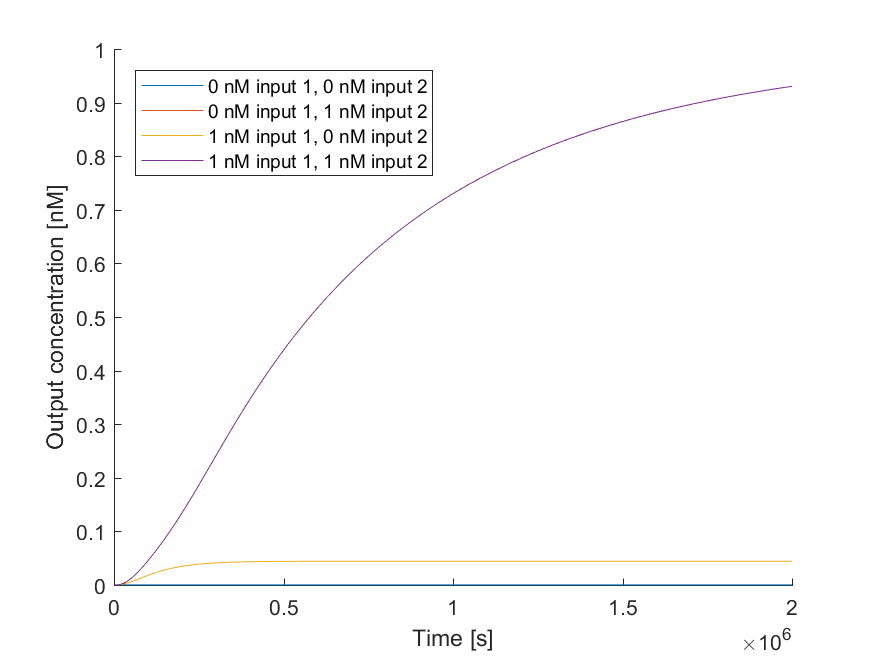
\includegraphics[width=\textwidth]{images/and_simulation.png}
\caption{Time analysis of the 2-input AND.}
\end{subfigure}
\caption{Simulation results of the trained 2-input AND gate. The network is trained to activate when both of the inputs are active. The correct output was obtained after 21 iterations of the training algorithm, with a weight of 1.9 for all inputs, and a threshold of 10.}
\label{2_and}
\end{figure}

\subsection{2-input OR}

\begin{figure}[H]
  \begin{subfigure}[t]{.49\columnwidth}

      \centering
    \begin{tabular}[b]{ccc}
      \hline
    \multicolumn{1}{l}{\textbf{Input 1}} & \multicolumn{1}{l}{\textbf{Input 2}} & \multicolumn{1}{l}{\textbf{Output}} \\
    \hline
    0                                    & 0                                    & 0                                   \\
    0                                    & 1                                    & 1                                   \\
    1                                    & 0                                    & 1                                   \\
    1                                    & 1                                    & 1 \\
    \hline
    \end{tabular}
    \caption{Truth table for the 2-input OR gate.}
\end{subfigure}
\begin{subfigure}[t]{.49\textwidth}
  \includegraphics[width=\textwidth]{figures/trained_2_or.tikz}
  \caption{Diagram of the 2-input OR with correct weights and threshold.}
\end{subfigure}
\hfill
\begin{subfigure}[t]{\textwidth}
  \centering
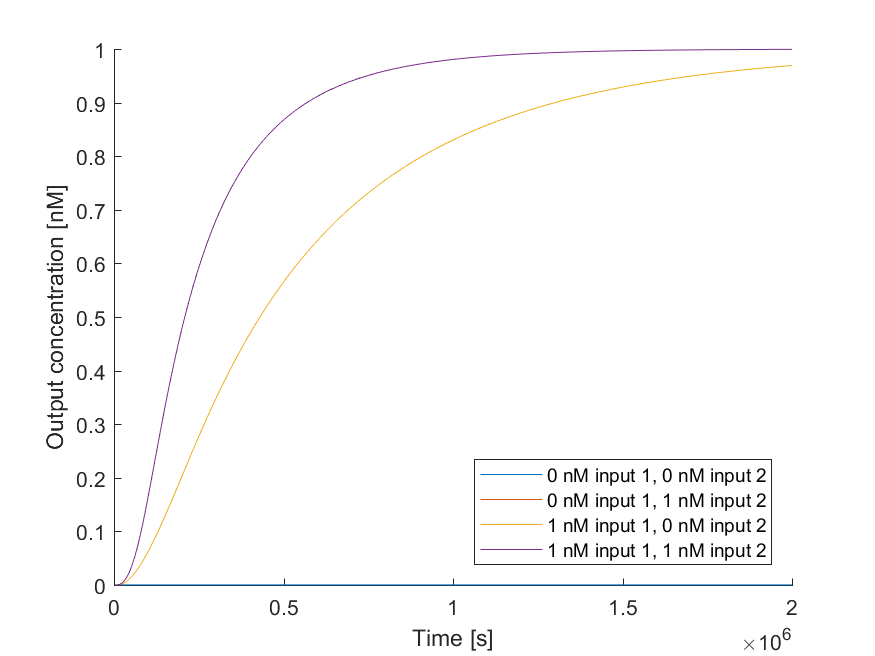
\includegraphics[width=\textwidth]{images/or_simulation.png}
\caption{Time analysis of the 2-input OR.}
\end{subfigure}
\caption{Simulation results of the trained 2-input OR gate. The network is trained to activate when one of the inputs is active. The correct output was obtained after 22 iterations of the training algorithm, with a weight of 2.1 for all inputs, and a threshold of 10.}
\label{2_or}
\end{figure}

\subsection{3-input AND}

\begin{figure}[H]
  \begin{subfigure}[t]{.49\columnwidth}
    \begin{adjustbox}{width=\textwidth}
    \begin{tabular}[b]{cccc}
      \hline
    \multicolumn{1}{l}{\textbf{Input 1}} & \multicolumn{1}{l}{\textbf{Input 2}} & \multicolumn{1}{l}{\textbf{Input 3}} & \multicolumn{1}{l}{\textbf{Output}} \\
    \hline
    0 & 0                                    & 0                                    & 0                                   \\
    0 & 0                                    & 1                                    & 0                                   \\
    0 & 1                                    & 0                                    & 0                                   \\
    0 & 1                                    & 1                                    & 0                                   \\
    1 & 0                                    & 0                                    & 0                                   \\
    1 & 0                                    & 1                                    & 0                                   \\
    1 & 1                                    & 0                                    & 0                                   \\
    1 & 1                                    & 1                                    & 1                                   \\

    \hline
    \end{tabular}
  \end{adjustbox}
    \caption{Truth table for the 3-input AND gate.}
\end{subfigure}
\begin{subfigure}[t]{.49\textwidth}
  \includegraphics[width=\textwidth]{figures/trained_3_and.tikz}
  \caption{Diagram of the 3-input AND with correct weights and threshold.}
\end{subfigure}
\hfill
\begin{subfigure}[t]{\textwidth}
  \centering
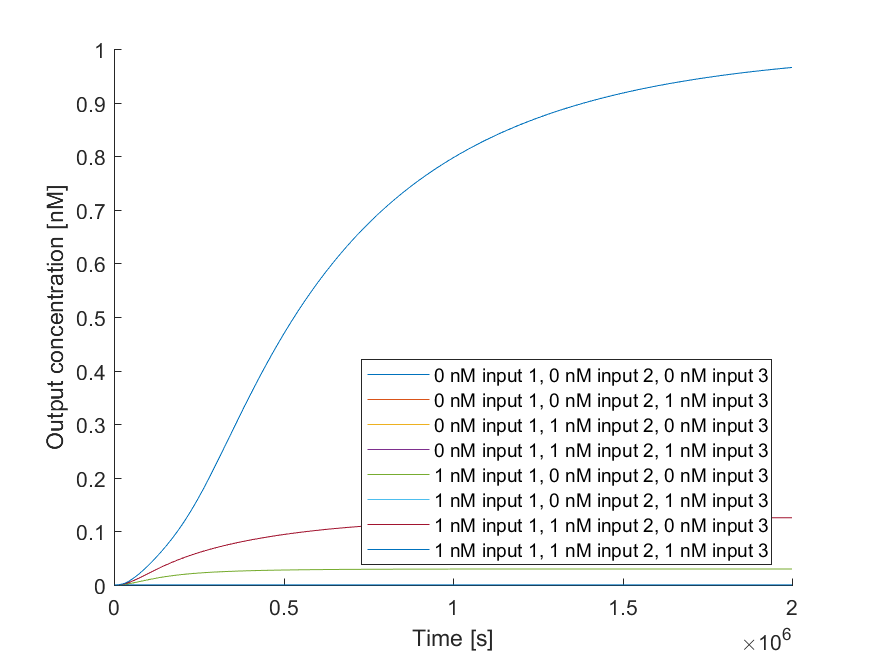
\includegraphics[width=\textwidth]{images/and_simulation_3input.png}
\caption{Time analysis of the 3-input AND.}
\end{subfigure}
\caption{Simulation results of the trained 3-input AND gate. The network is trained to activate when all of the inputs are active. The correct output was obtained after 14 iterations of the training algorithm, with a weight of 1.2 for all inputs, and a threshold of 10.}
\label{3_and}
\end{figure}

\subsection{3-input 1-OR}

\begin{figure}[H]
  \begin{subfigure}[t]{.49\columnwidth}

      \begin{adjustbox}{width=\textwidth}
    \begin{tabular}[b]{cccc}
      \hline
    \multicolumn{1}{l}{\textbf{Input 1}} & \multicolumn{1}{l}{\textbf{Input 2}} & \multicolumn{1}{l}{\textbf{Input 3}} & \multicolumn{1}{l}{\textbf{Output}} \\
    \hline
    0 & 0                                    & 0                                    & 0                                   \\
    0 & 0                                    & 1                                    & 1                                   \\
    0 & 1                                    & 0                                    & 1                                   \\
    0 & 1                                    & 1                                    & 1                                   \\
    1 & 0                                    & 0                                    & 1                                   \\
    1 & 0                                    & 1                                    & 1                                   \\
    1 & 1                                    & 0                                    & 1                                   \\
    1 & 1                                    & 1                                    & 1                                   \\

    \hline
    \end{tabular}
  \end{adjustbox}
    \caption{Truth table for the 3-input 1-OR gate.}
\end{subfigure}
\begin{subfigure}[t]{.49\textwidth}
  \includegraphics[width=\textwidth]{figures/trained_3_1_or.tikz}
  \caption{Diagram of the 3-input 1-OR with correct weights and threshold.}
\end{subfigure}
\hfill
\begin{subfigure}[t]{\textwidth}
  \centering
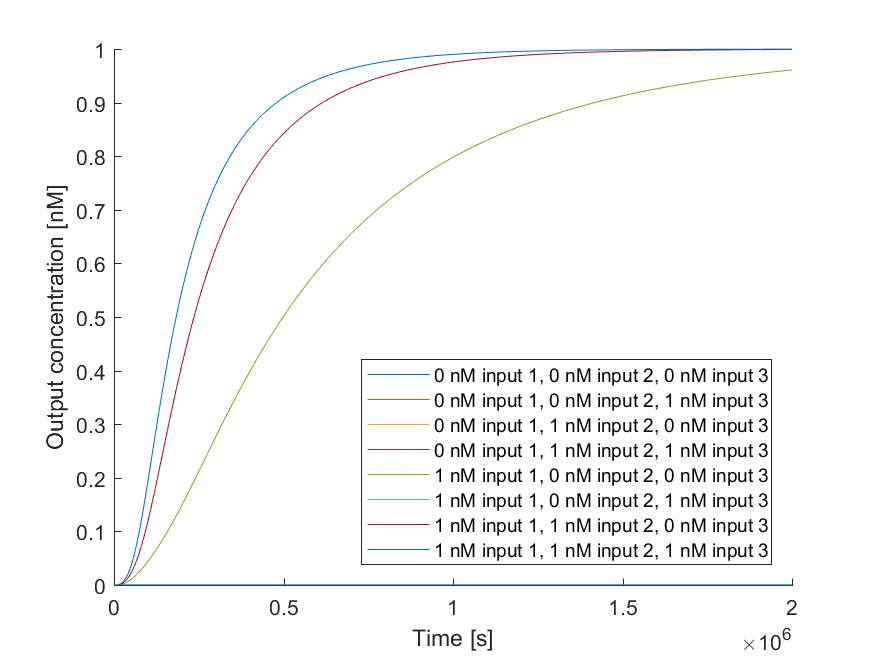
\includegraphics[width=\textwidth]{images/or_1_simulation_3input.png}
\caption{Time analysis of the 3-input 1-OR.}
\end{subfigure}
\caption{Simulation results of the trained 3-input 1-OR gate. The network is trained to activate when at least 1 of the inputs is active. The correct output was obtained after 16 iterations of the training algorithm, with a weight of 1.3 for all inputs, and a threshold of 10.}
\label{3_1_or}
\end{figure}

\subsection{3-input 2-OR}


\begin{figure}[H]
  \begin{subfigure}[t]{.49\columnwidth}
    \begin{adjustbox}{width=\textwidth}
    \begin{tabular}[b]{cccc}
      \hline
    \multicolumn{1}{l}{\textbf{Input 1}} & \multicolumn{1}{l}{\textbf{Input 2}} & \multicolumn{1}{l}{\textbf{Input 3}} & \multicolumn{1}{l}{\textbf{Output}} \\
    \hline
    0 & 0                                    & 0                                    & 0                                   \\
    0 & 0                                    & 1                                    & 0                                   \\
    0 & 1                                    & 0                                    & 0                                   \\
    0 & 1                                    & 1                                    & 1                                   \\
    1 & 0                                    & 0                                    & 0                                   \\
    1 & 0                                    & 1                                    & 1                                   \\
    1 & 1                                    & 0                                    & 1                                   \\
    1 & 1                                    & 1                                    & 1                                   \\

    \hline
    \end{tabular}
  \end{adjustbox}
    \caption{Truth table for the 3-input 2-OR gate.}
\end{subfigure}
\begin{subfigure}[t]{.49\textwidth}
  \includegraphics[width=\textwidth]{figures/trained_3_2_or.tikz}
  \caption{Diagram of the 3-input 2-OR with correct weights and threshold.}
\end{subfigure}
\hfill
\begin{subfigure}[t]{\textwidth}
  \centering
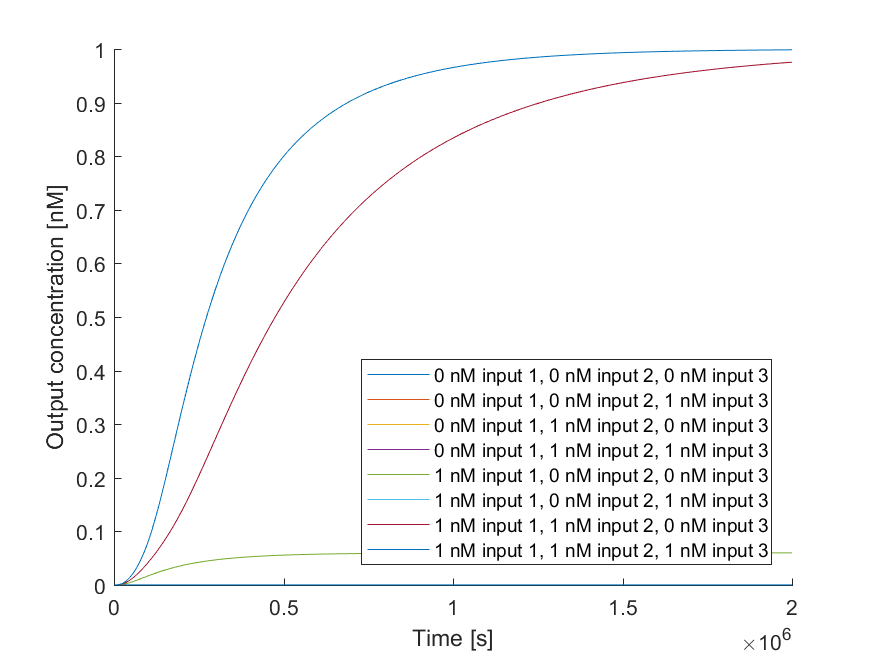
\includegraphics[width=\textwidth]{images/or_2_simulation_3input.png}
\caption{Time analysis of the 3-input 2-OR.}
\end{subfigure}
\caption{Simulation results of the trained 3-input 2-OR gate. The network is trained to activate when at least 2 of the inputs is active. The correct output was obtained after 15 iterations of the training algorithm, with a weight of 1.4 for all inputs, and a threshold of 10.}
\label{3_2_or}
\end{figure}

\section{Translation}
The gels from the transcription, annealing, and PCR reactions is shown here. As it was not possible to get the correct RNA sequences needed for fluorescence measurements, there are no strand displacement results to compare with the results from the original article \cite{Picuri2009}.

\begin{figure}[h]
\begin{subfigure}[t]{0.54\textwidth}
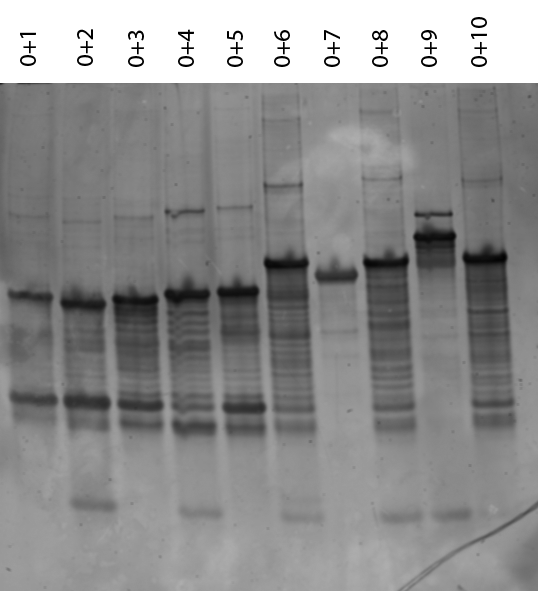
\includegraphics[width=\textwidth]{images/promoter_annealing_gel.png}
\caption{}
\label{promoter_annealing_gel}
\end{subfigure}
\begin{subfigure}[t]{0.46\textwidth}
  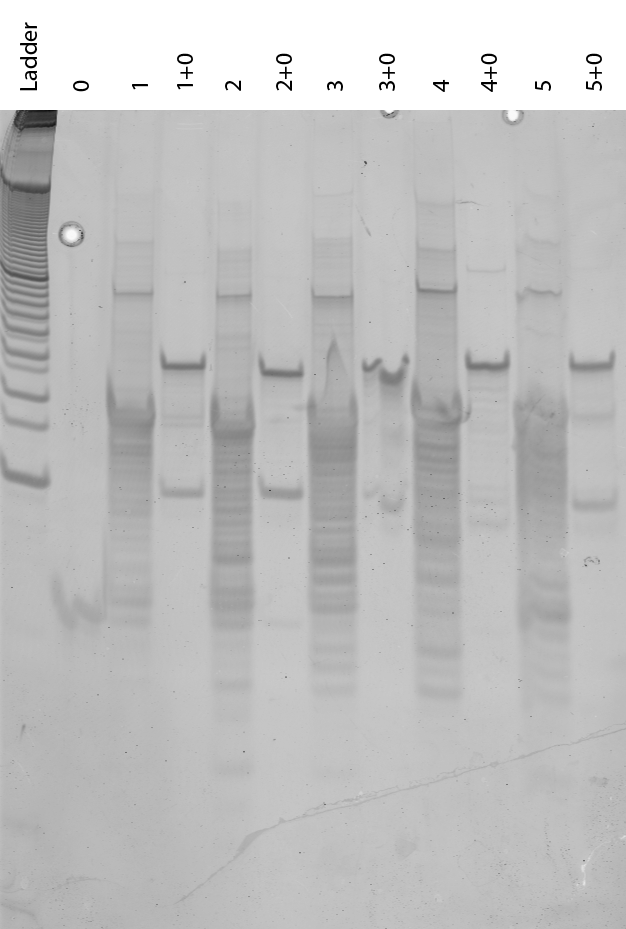
\includegraphics[width=\textwidth]{images/translator_annealing_2.png}
  \caption{}
  \label{translator_annealing_2}
\end{subfigure}
\caption{\subref{promoter_annealing_gel} Typhoon scan of SYBR Gold stained native PAGE gel, with the annealed templates and promoter strands. The lanes are labelled by which strands are annealed (see table \ref{dna_strands}). \subref{translator_annealing_2} The annealed oligos together with controls and a 10 nt ladder. The lanes are labelled with the oligo names given in \tref{dna_strands}. The plus symbol denotes which strands are annealed.}
\end{figure}

\begin{figure}[h]
  \begin{subfigure}[t]{0.49\textwidth}
  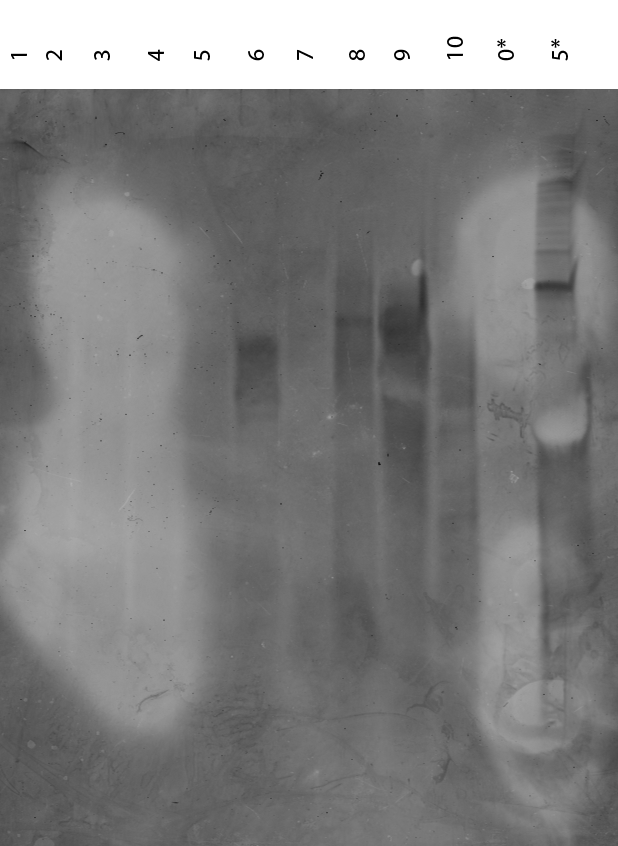
\includegraphics[width=\textwidth]{images/translator_transcription_1.png}
  \caption{}
  \label{transcription_1}
  \end{subfigure}
  \begin{subfigure}[t]{0.49\textwidth}
    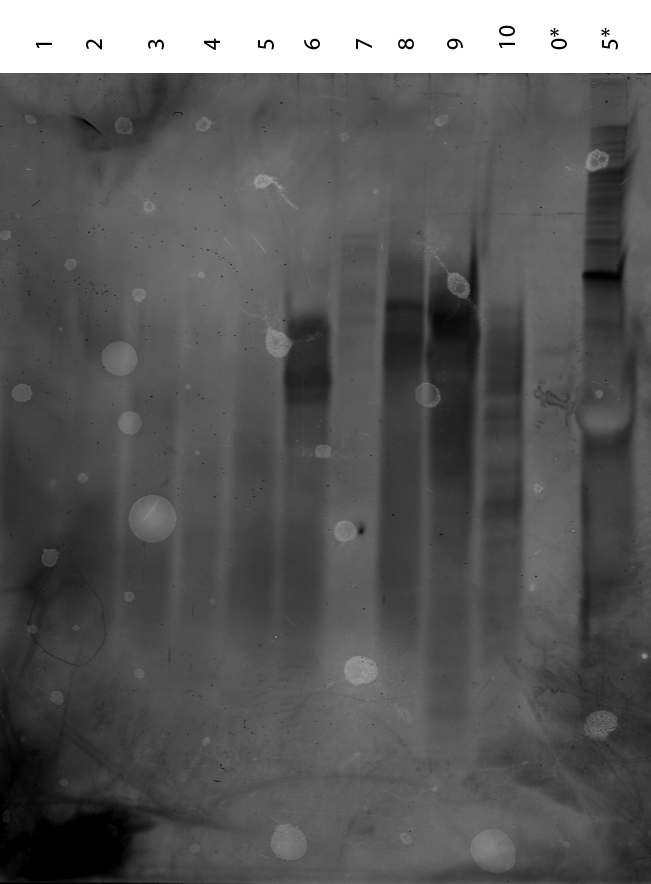
\includegraphics[width=\textwidth]{images/translator_transcription_2.png}
    \caption{}
    \label{transcription_2}
  \end{subfigure}
  \caption{\subref{transcription_1} Typhoon scan of SYBR Gold stained native PAGE gel, with the transcribed RNA strands in lanes 1-10, and controls in 11 and 12. The lanes are labelled by which strands are annealed (see \tref{rna_strands}). The asterix refers to the DNA strands in \tref{dna_strands}. \subref{transcription_2} The same gel after further staining in SYBR Gold.}
\end{figure}

\begin{figure}[h]
\begin{subfigure}[t]{.43\textwidth}
  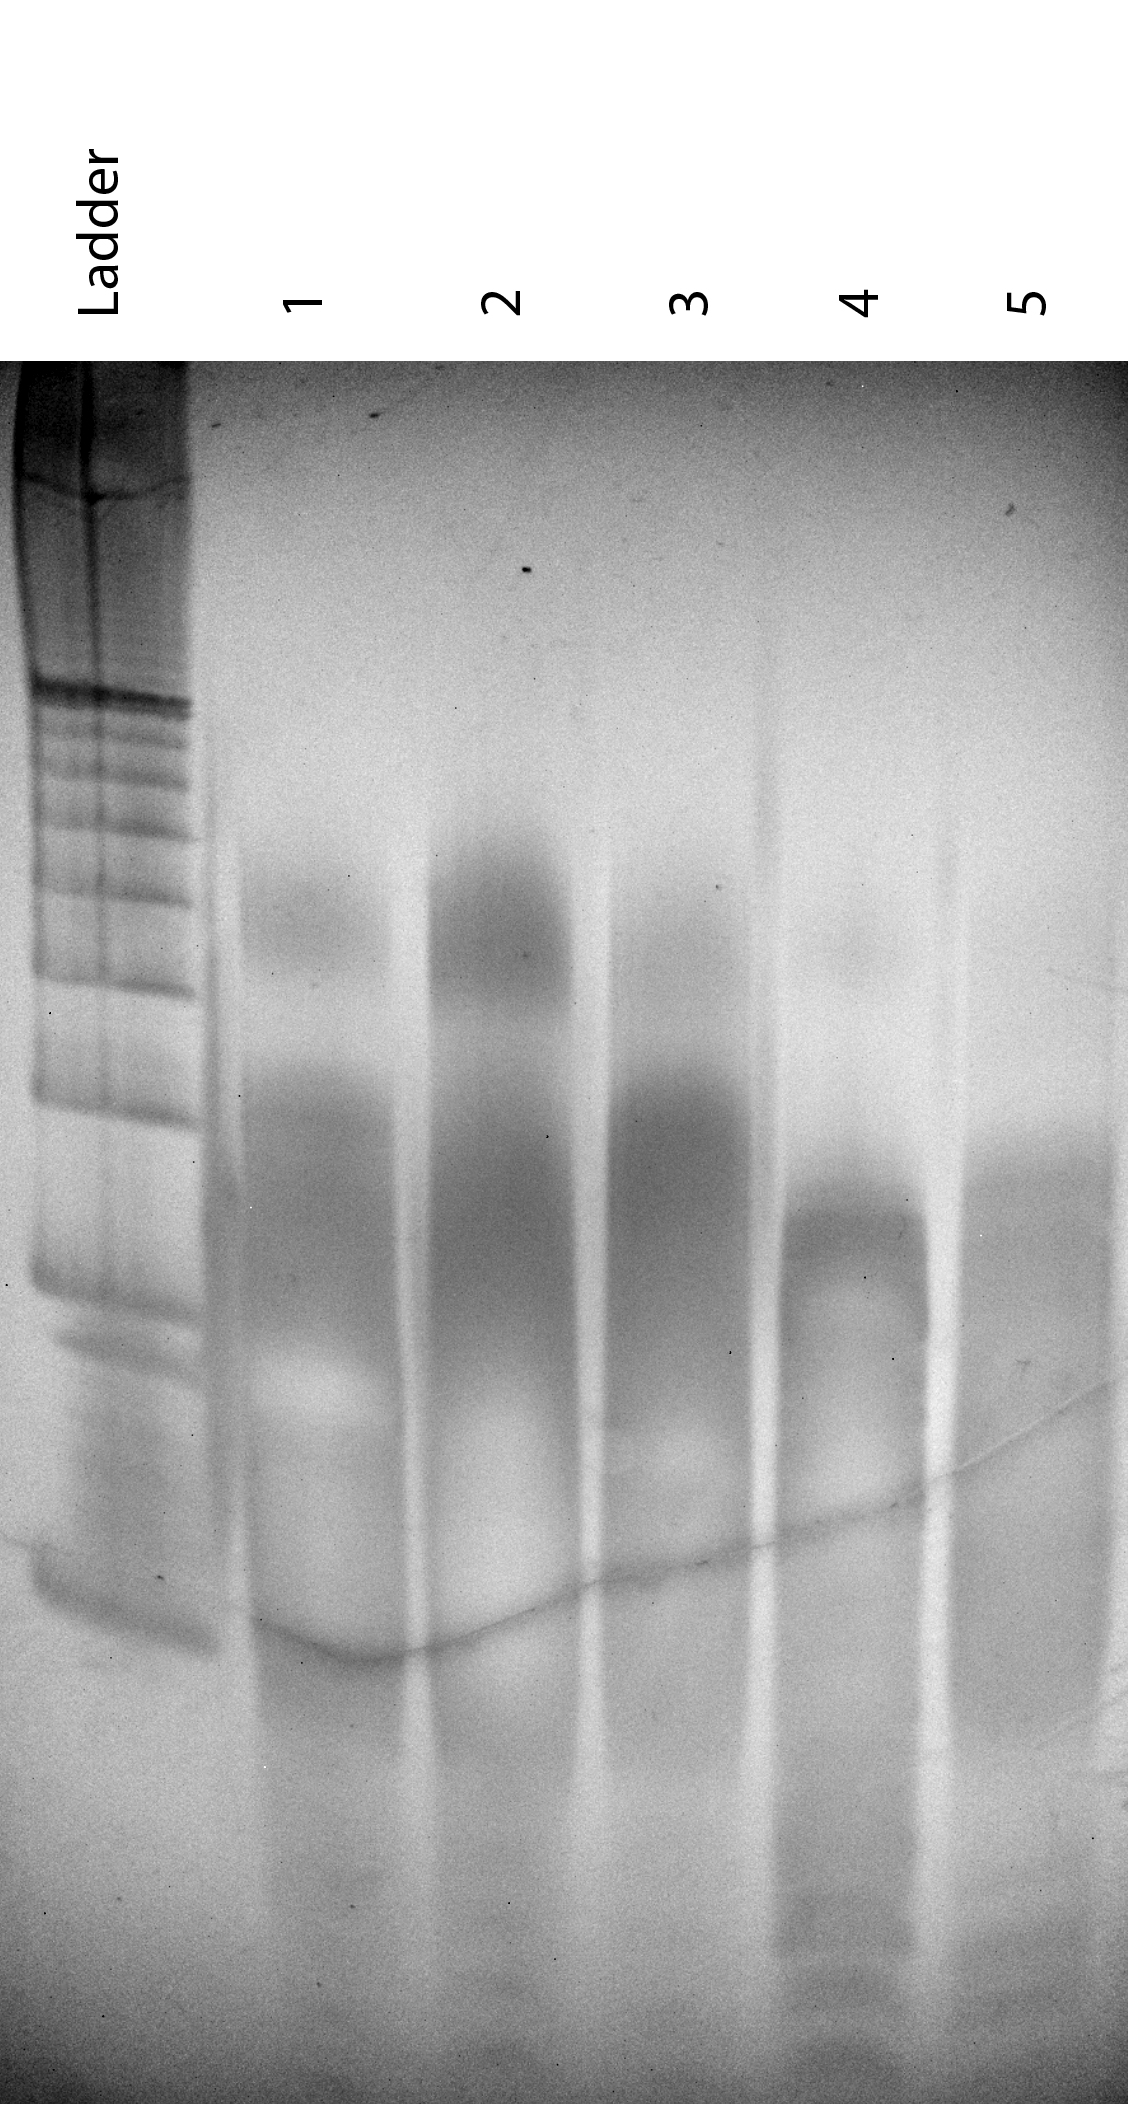
\includegraphics[width=\textwidth]{images/translator_transcription_3.png}
  \caption{}
  \label{translator_transcription_3}
\end{subfigure}
\begin{subfigure}[t]{.55\textwidth}
  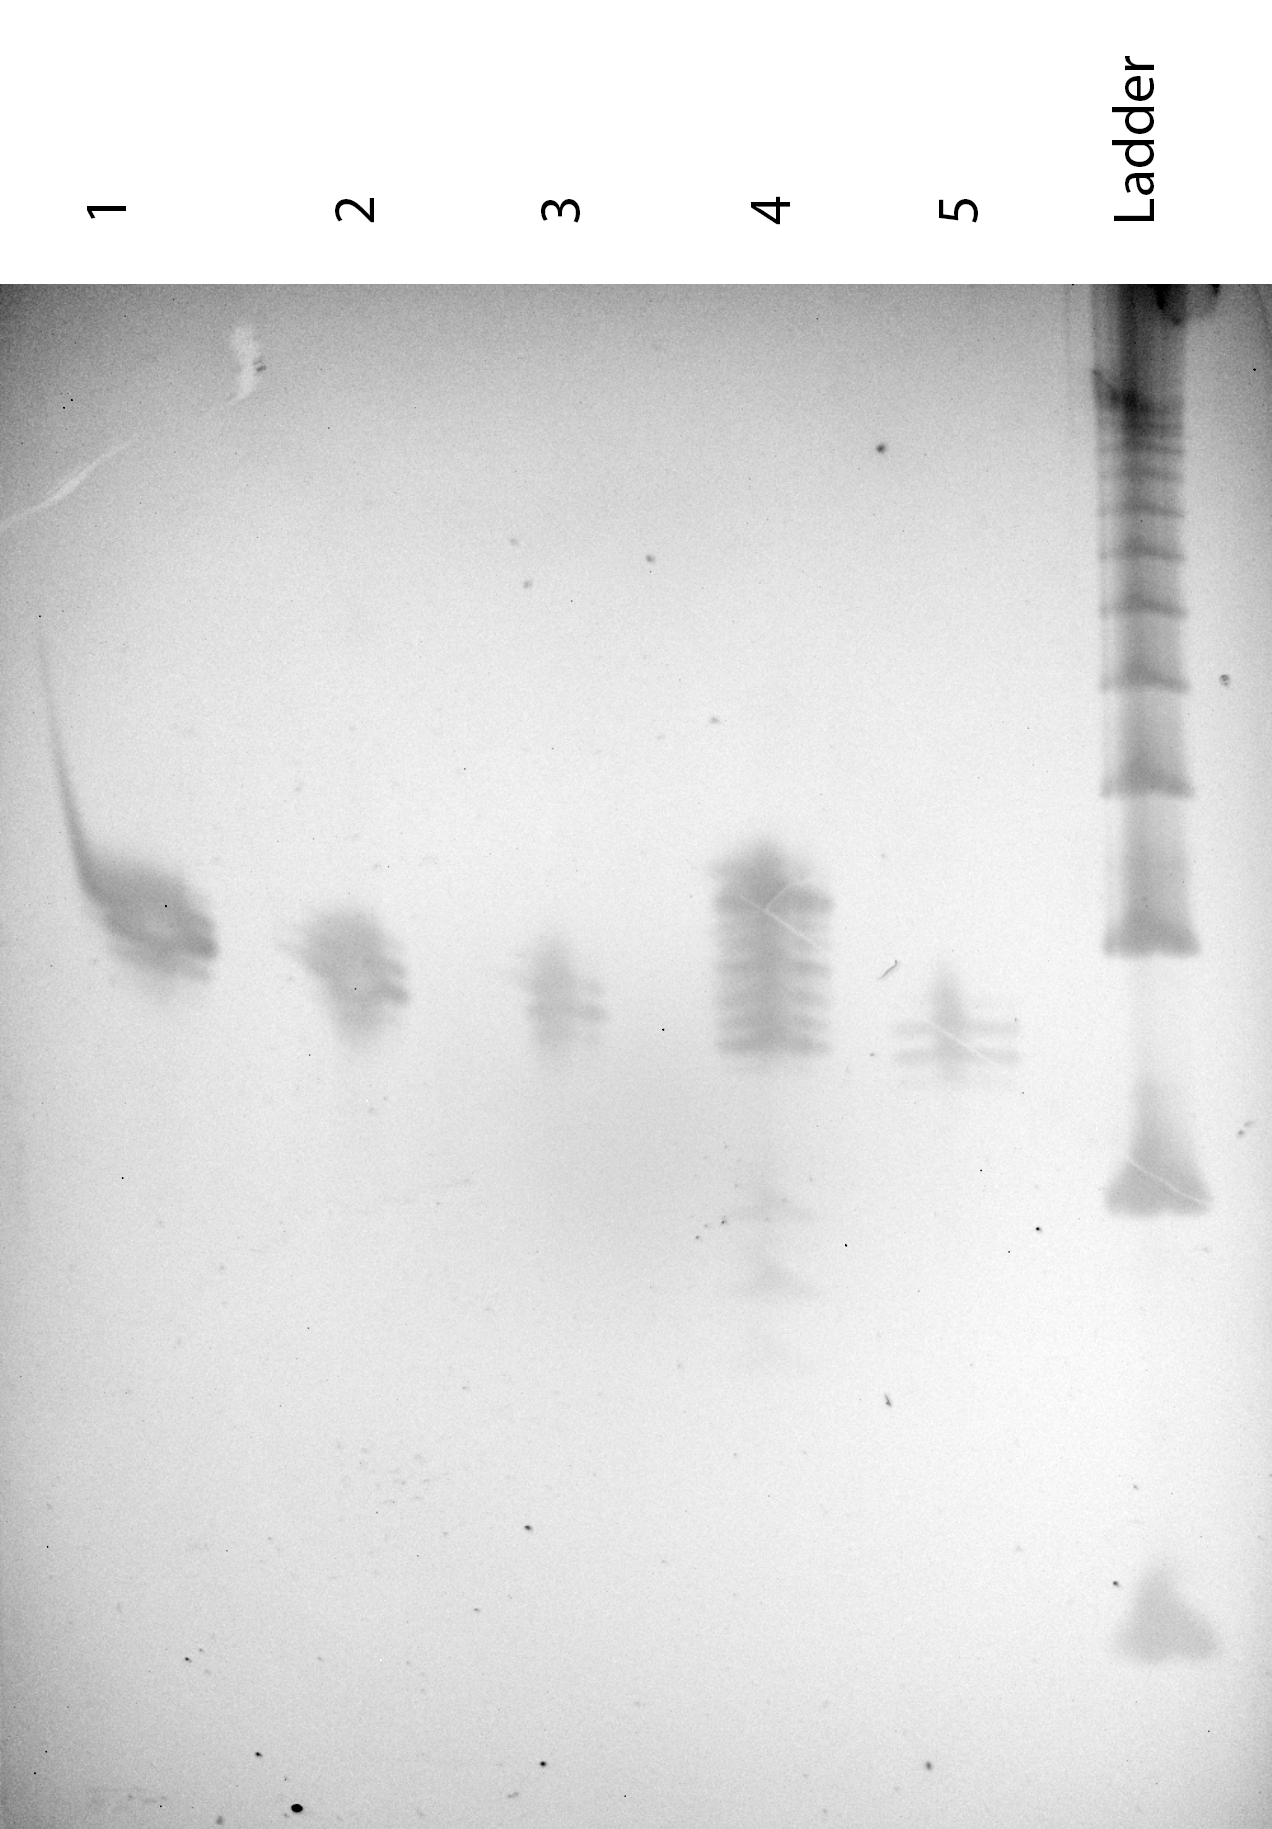
\includegraphics[width=\textwidth]{images/translator_transcription_purified.png}
  \caption{}
  \label{translator_transcription_purified}
\end{subfigure}
\caption{\subref{translator_transcription_3} The transcribed short translator sequences and a 10 nt ladder. The lanes are labelled with the oligo names given in \tref{rna_strands}. \subref{translator_transcription_purified} The purified short translator RNA oligos.}
\end{figure}

\begin{figure}[h]
\begin{subfigure}[t]{.5\textwidth}
  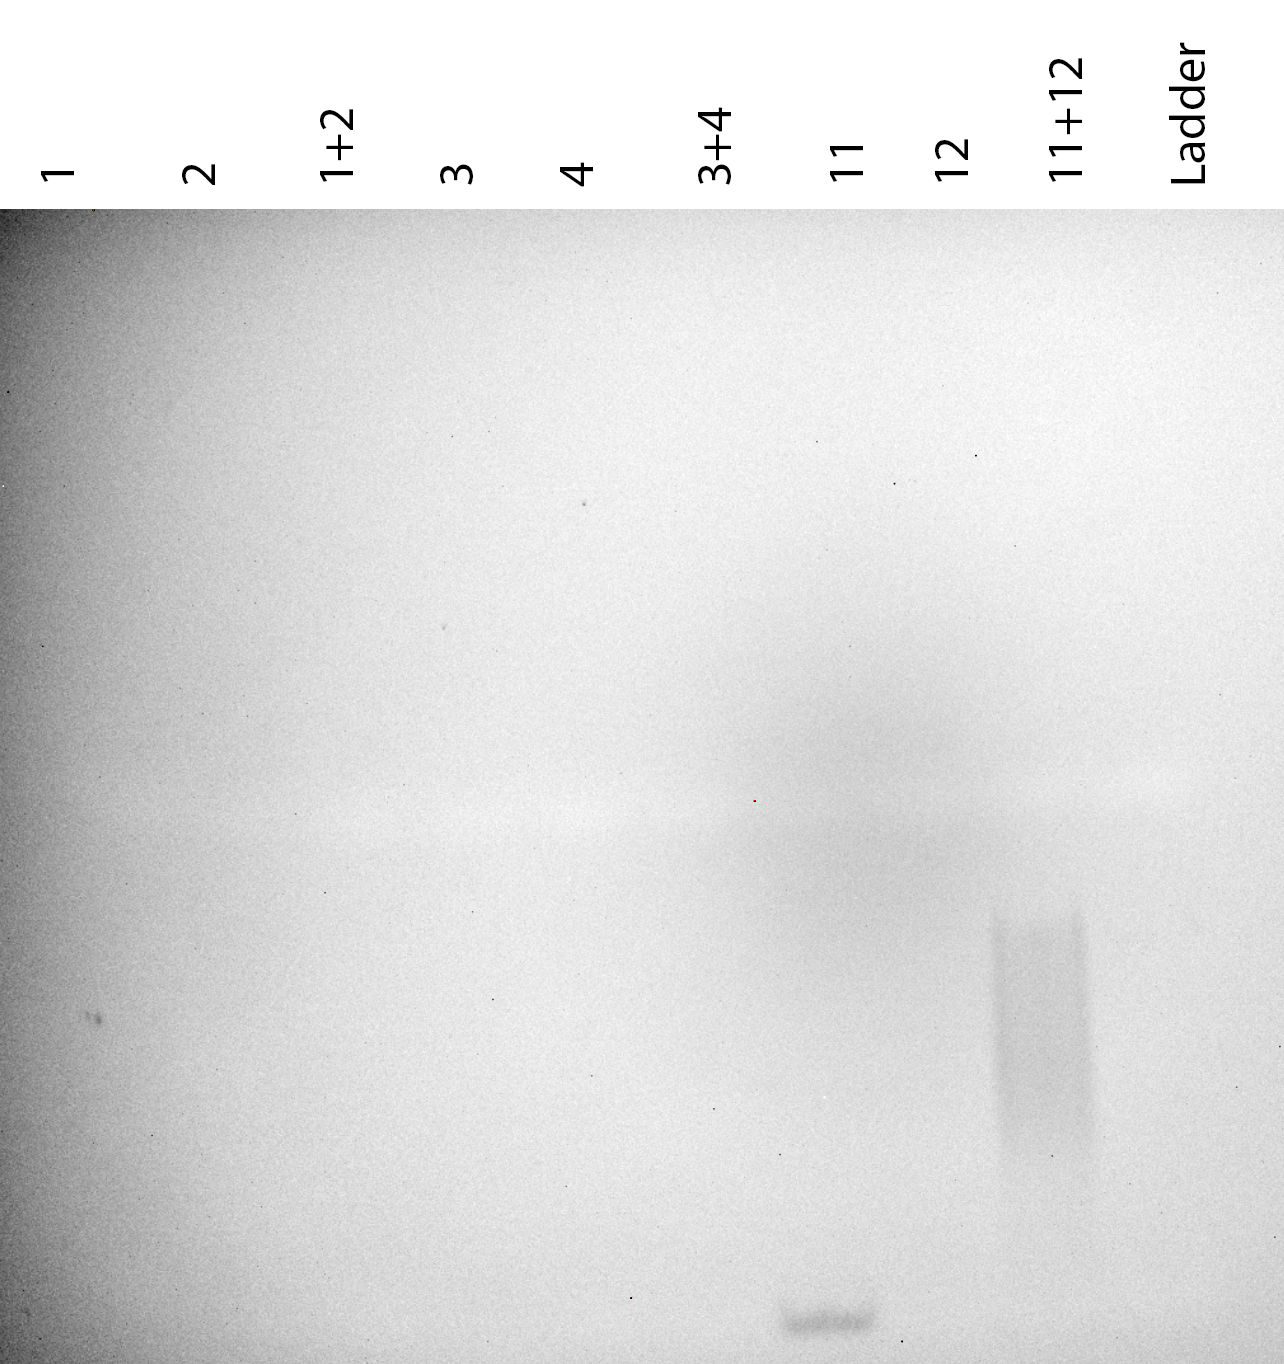
\includegraphics[width=\textwidth]{images/transcription_annealed_nostain.png}
  \caption{Not stained}
  \label{transcription_annealed_nostain}
\end{subfigure}
\begin{subfigure}[t]{.5\textwidth}
  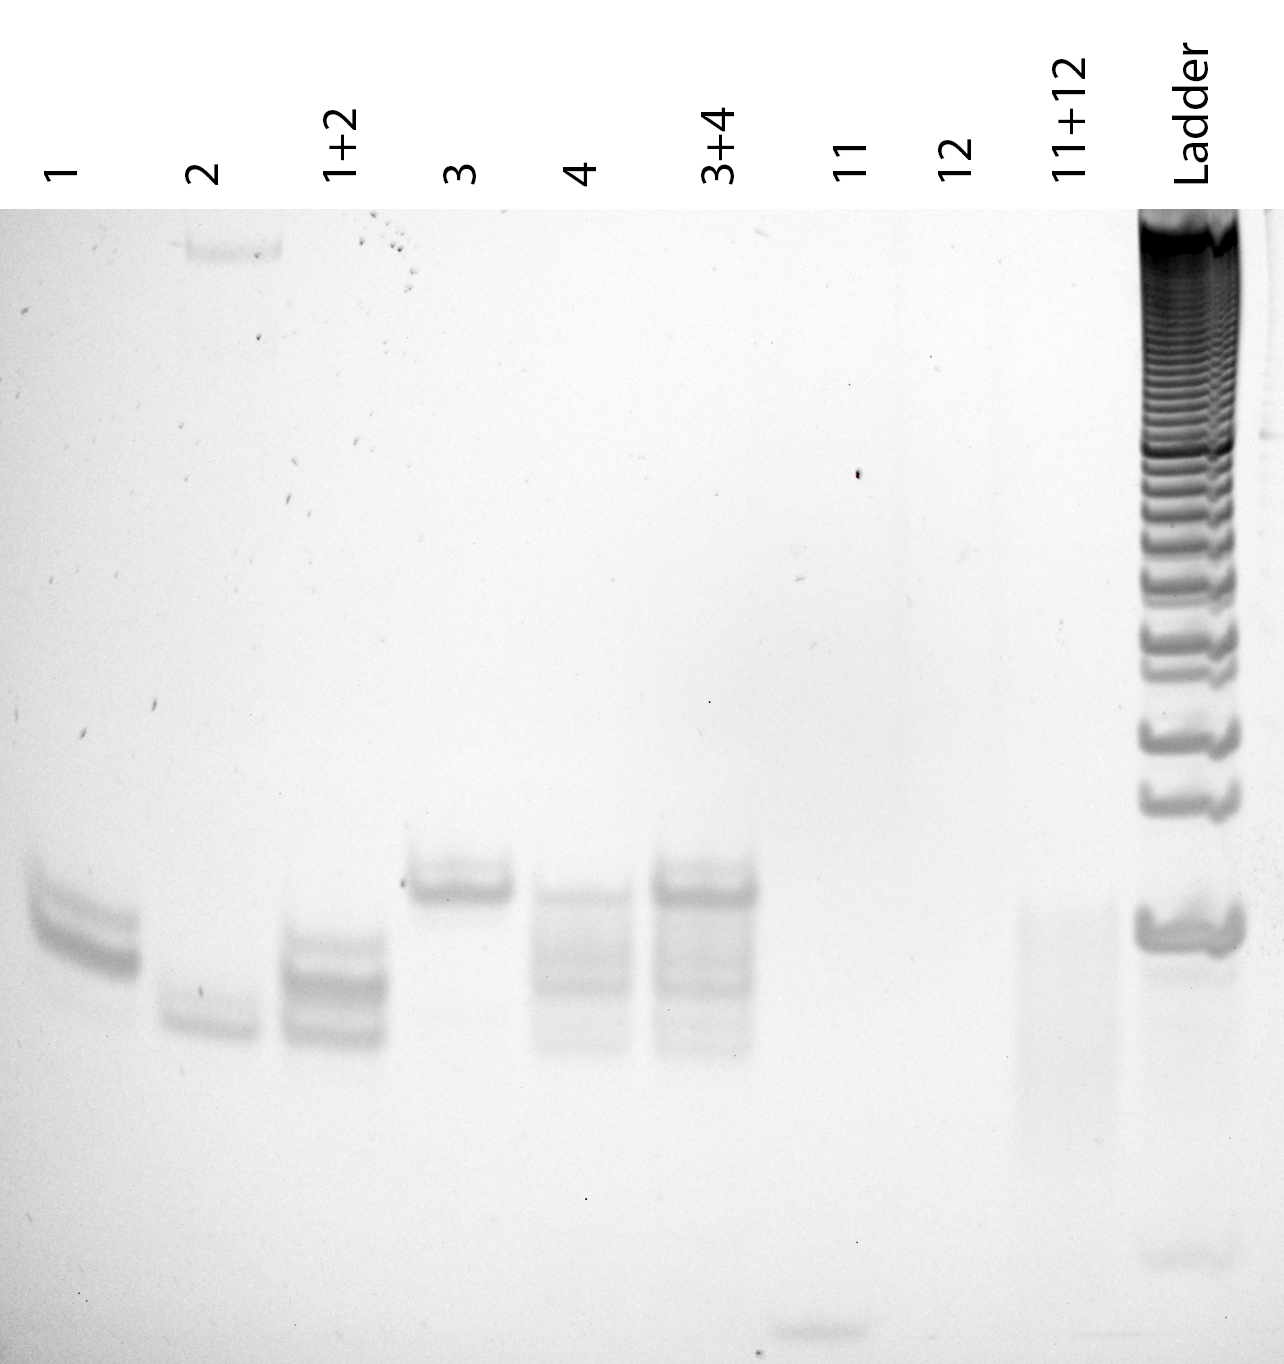
\includegraphics[width=\textwidth]{images/transcription_annealed_stain.png}
  \caption{Stained}
  \label{transcription_annealed_stain}
\end{subfigure}
\caption{The annealed short translator subunits and reporter, with the single strands as controls, and a 10 nt ladder.}
\label{transcription_annealed}
\end{figure}

\begin{figure}[h]
\begin{subfigure}[t]{0.51\textwidth}
  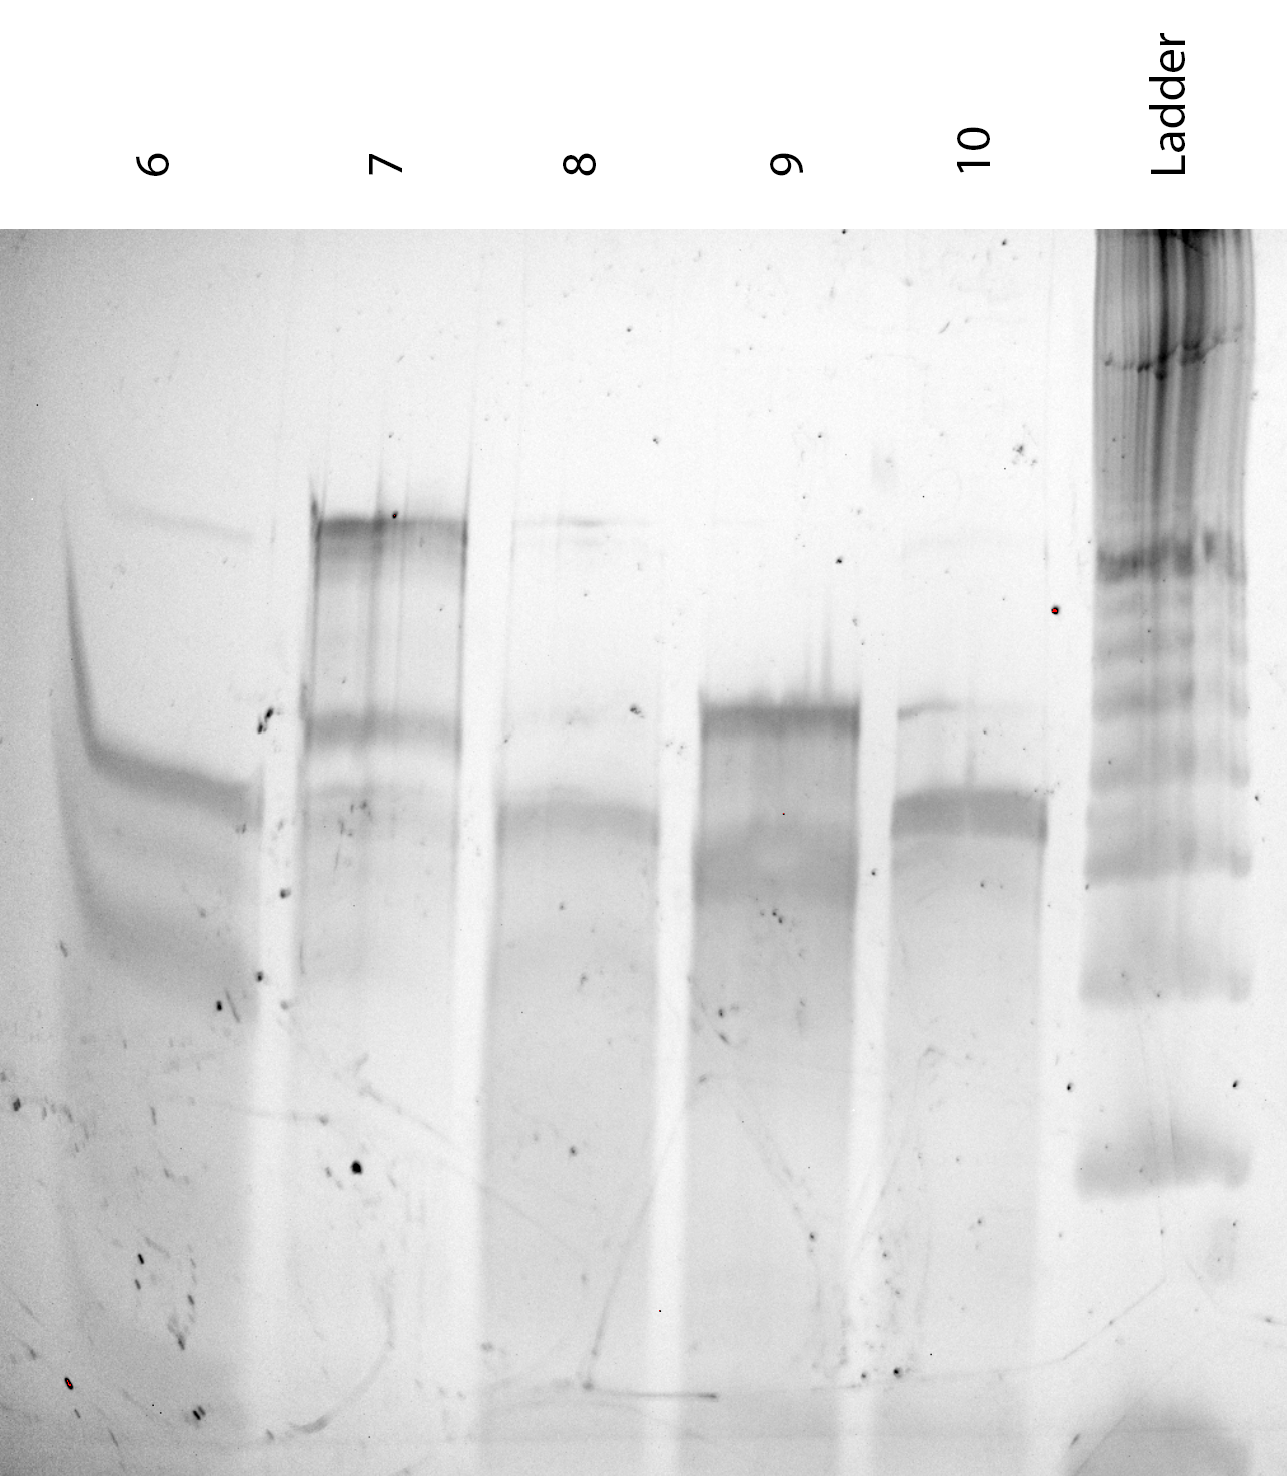
\includegraphics[width=\textwidth]{images/translator_transcription_long_1.png}
  \caption{}
  \label{translator_transcription_long_1}
\end{subfigure}
\begin{subfigure}[t]{0.49\textwidth}
  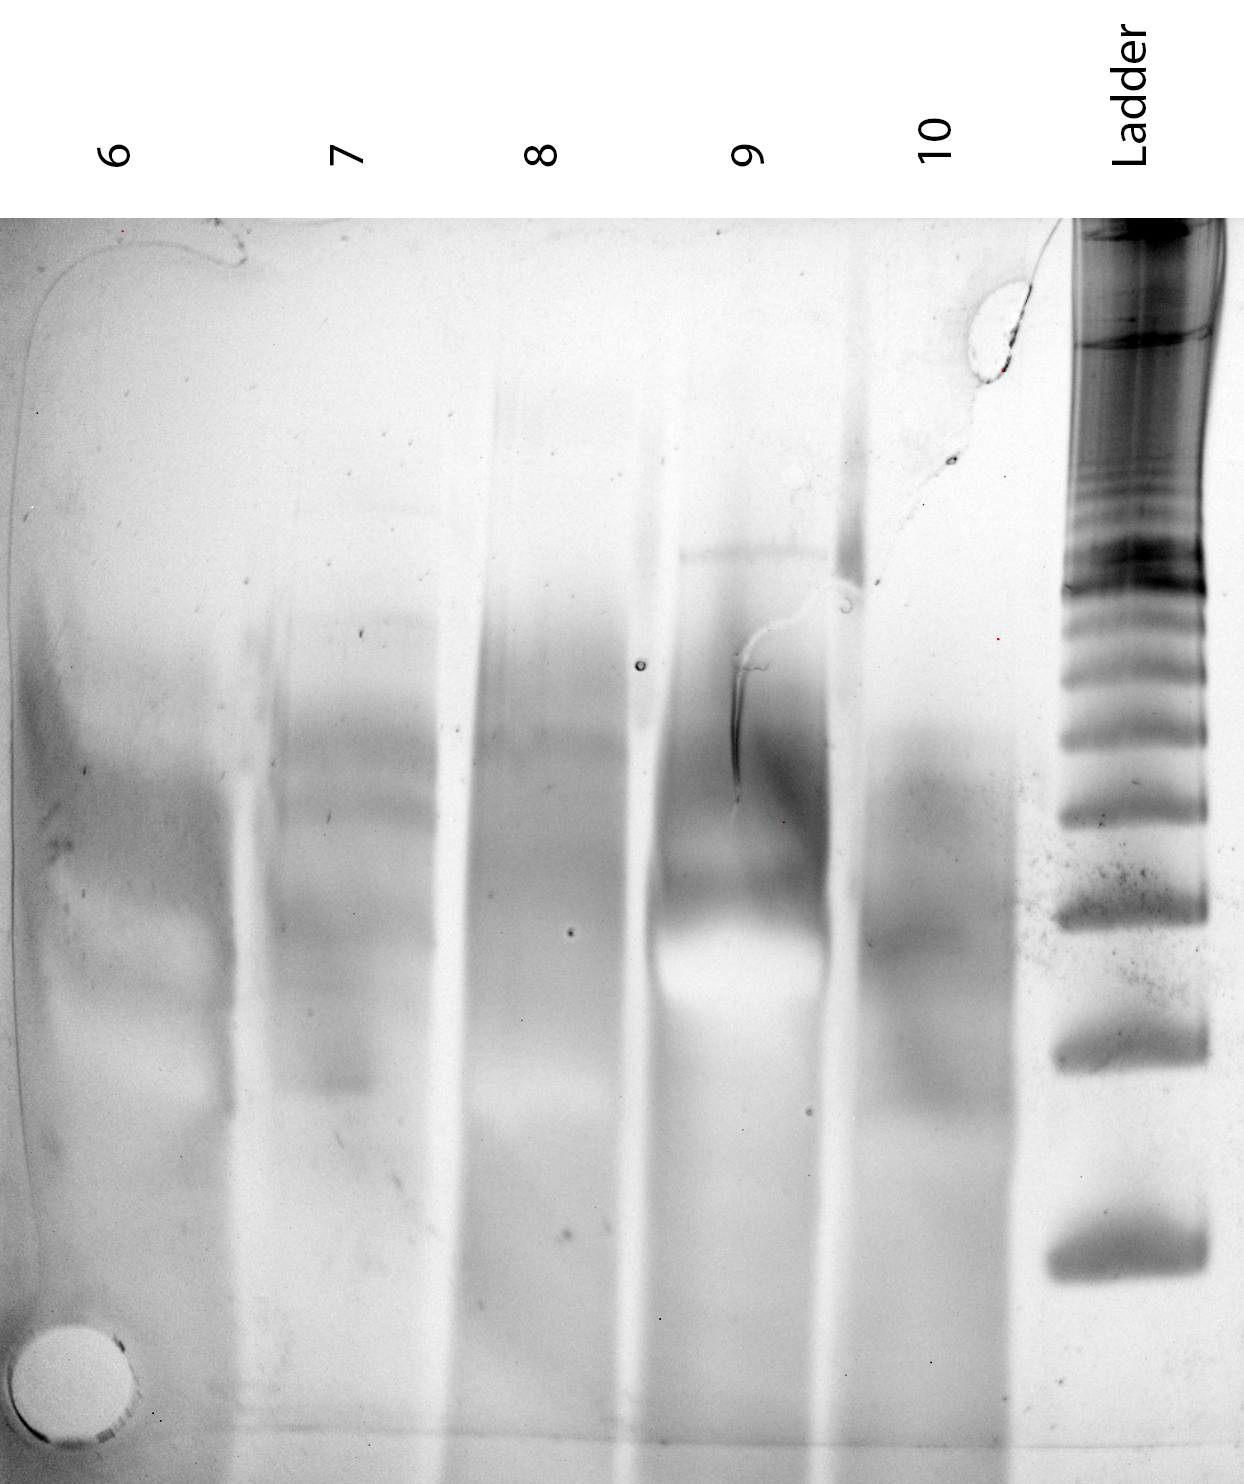
\includegraphics[width=\textwidth]{images/translator_transcription_long_2.png}
  \caption{}
  \label{translator_transcription_long_2}
\end{subfigure}
\caption{\subref{translator_transcription_long_1} Transcription of the long translator sequences with a 10 nt ladder. \subref{translator_transcription_long_2} Transcription of the long translator sequences with a 10 nt ladder, using an adapted protocol.}
\end{figure}

\begin{figure}[h]
\begin{subfigure}[t]{0.53\textwidth}
  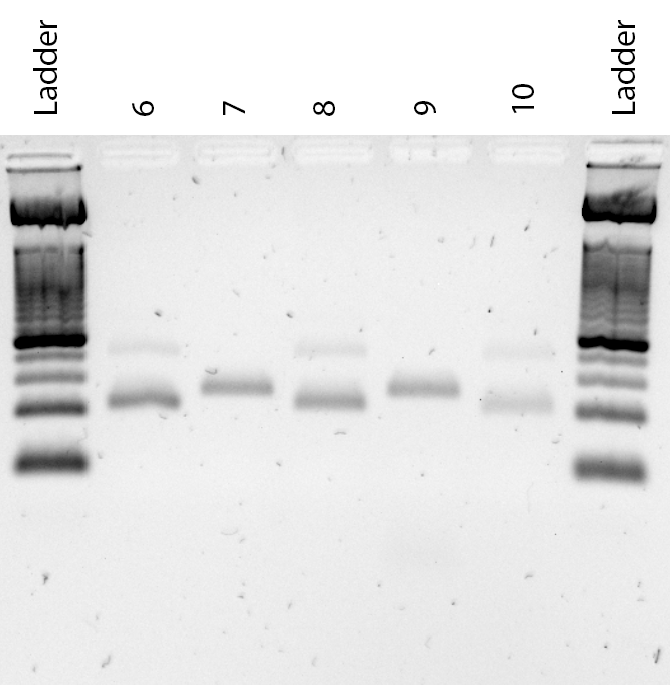
\includegraphics[width=\textwidth]{images/translator_pcr_long_1.png}
  \caption{}
  \label{translator_pcr_long_1}
\end{subfigure}
\begin{subfigure}[t]{0.47\textwidth}
  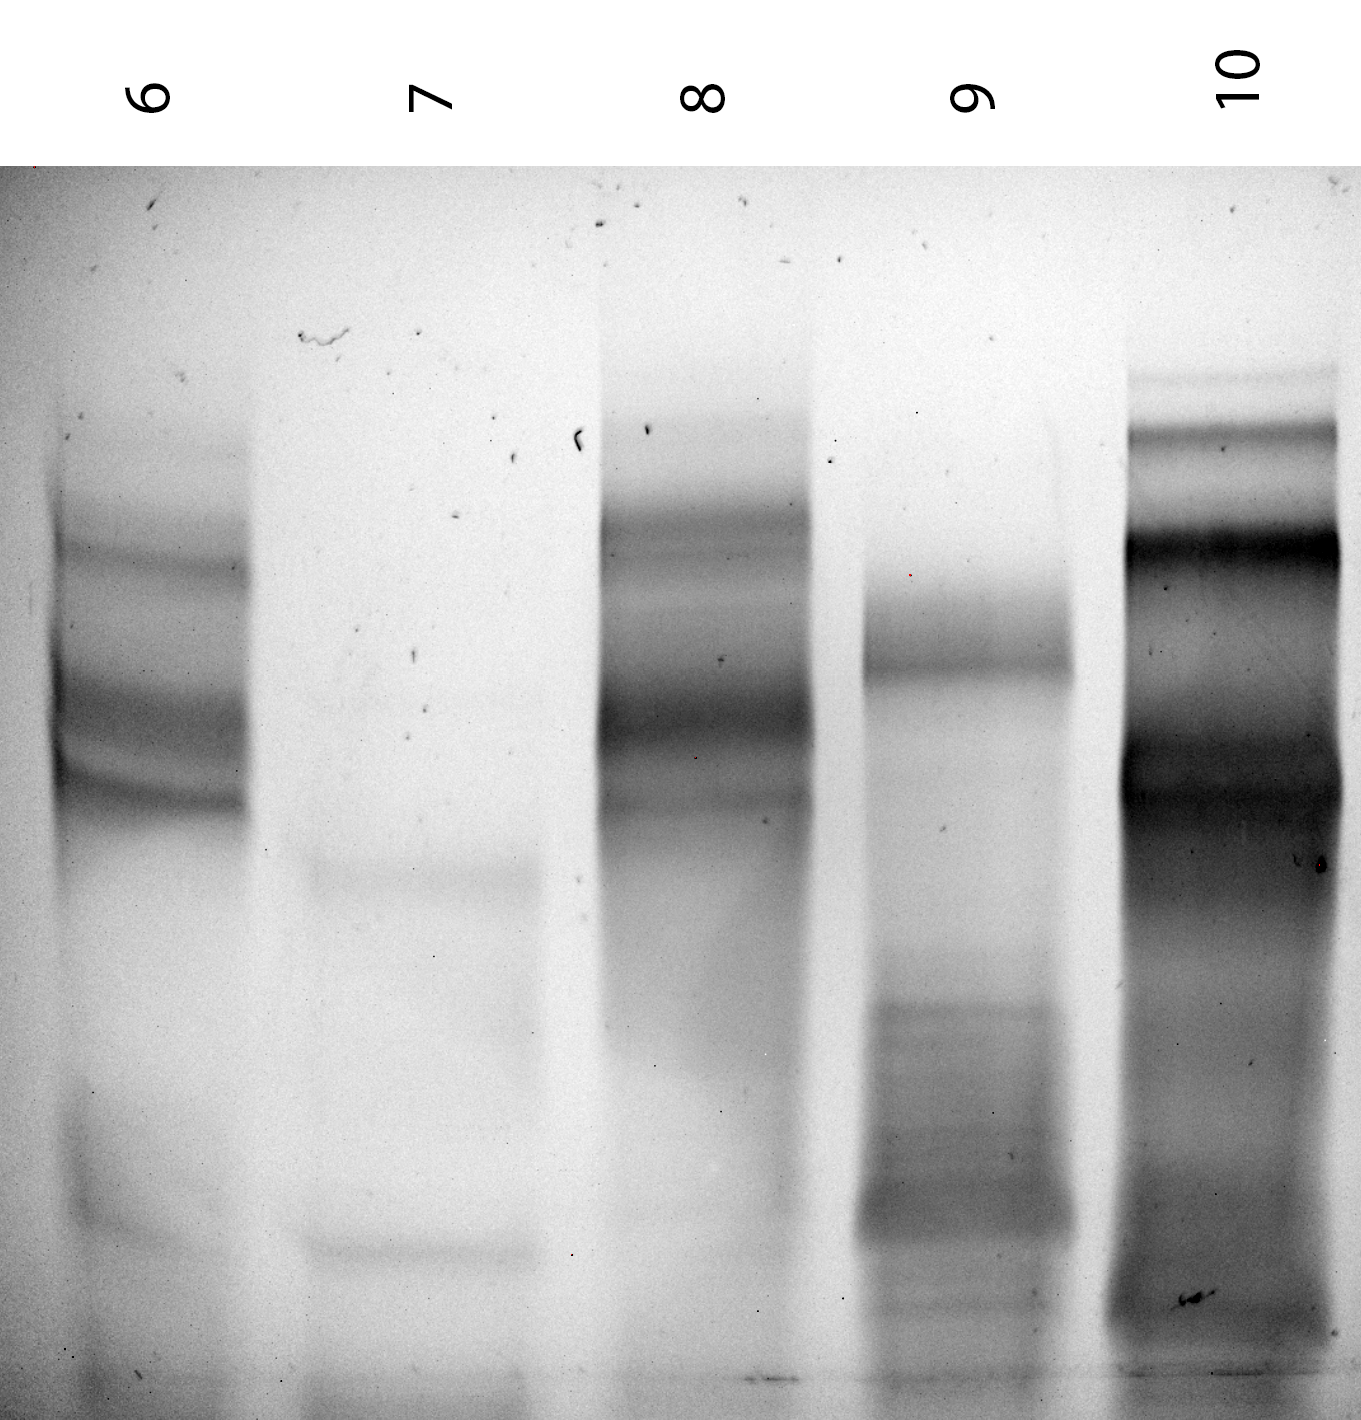
\includegraphics[width=\textwidth]{images/translator_transcription_long_ds_1.png}
  \caption{}
  \label{translator_transcription_long_ds_1}
\end{subfigure}
\caption{\subref{translator_pcr_long_1} PCR product of the long translator sequences. \subref{translator_transcription_long_ds_1} Transcription of the double-stranded long translator sequences.}
\end{figure}
